

%Models for object detection

\section{Object detection component implementation}\label{sec:object-detection-component-implementation}

\subsection{Dataset and formats}\label{subsec:dataset-and-formats}
My project started with choosing and downloading a suitable dataset containing data from urban traffic scenarios.
I chose the Cityscapes dataset~\cite{Cordts2016Cityscapes}.
These data was not in the correct format for the Yolo model to use.
The dataset contains semantic segmentations, but the vanilla Yolo architecture is working with bounding boxes.
I needed to write a format conversion script, following the descriptions in subsection \ref{subsec:data-management}.


\paragraph{Cityscapes:}\label{par:cityscapes}
the Cityscapes dataset is a large-scale dataset~\cite{Cordts2016Cityscapes} used for training and evaluating object detection models.
It contains high-resolution images of urban scenes, with detailed annotations for various objects such as cars,
pedestrians, and traffic signs.
The dataset is widely used in the field of computer vision for tasks such as semantic segmentation and object detection.


I chose the gtFine dataset, consisting precisely labelled segmentation masks.
Based on their work where they published this dataset~\cite{Cordts2016Cityscapes} titled \("\)he cityscapes dataset for semantic urban scene understanding\("\)
the gtFine dataset consists of 5000 images,
with a resolution of 1024\(\times\)2048 pixels, and annotations for 30 classes of objects.
It is divided into three subsets: training, validation, and test, with 2975, 500, and 1525 images, respectively.
The validation and training sets contain annotations for 30 classes, while the test set doesn't include any annotations.
The dataset is labelled using pixel-level segmentation masks, which provide detailed information about the
location and shape of objects in the scene.

However for the purpose of this work, the annotations were converted into bounding box format,
which is more suitable and straight forward for this object detection tasks.
Also, the dataset was filtered to include only the classes that are relevant to the project.

\subsection{Data engineering} \label{subsec:data-management}
The images and annotations are converted into a format that the Yolov8 model can process, which is
a text file containing the image path and the coordinates of the bounding boxes in pixels for each object in the image.
The format is straightforward: each line of the text file represents a single instance of an object.
The first variable is the label\_id, which denotes the object's class.
This is followed by the two-point's four \((x, y)\) type coordinates in pixel.
This process uses a custom script that reads the annotations from the Cityscapes dataset and converts the labels
into labels whose classes are filtered and transformed the relevant classes into the grouping I chose for this project.

The classes were grouped into five categories:
\begin{itemize}
    \item \textbf{small vehicle}~\textit{(usually cars, which are for personal use)},
    \item \textbf{large vehicle}~\textit{(busses, trucks and other large non personal vehicles)},
    \item \textbf{two wheeler}~\textit{(bicycles and motorcycles)},
    \item \textbf{On-rails}~\textit{(trains and trams though the smaller Fine dataset didn't include any in the training set)}
    \item and \textbf{person}~\textit{(pedestrian, and rider)}.
\end{itemize}

The categories were selected on the basis that the model's confusion is more readily managed when objects
that are more similar in appearance are grouped together, thereby facilitating the model's ability to
distinguish between them.

The script also converts the semantic segmentation masks into bounding boxes, trough finding the most
extreme points and of the mask, create a bounding box around them.
This converted output is then saved into a text file, which is in the format used as input for the Yolov8 model.

The final structure of the dataset with metadata (descriptors and lists of labels and pictures) is as follows:
\begin{itemize}
    \item \textbf{Root (gtFine)}: The root directory of the Cityscapes dataset, which contains the images and annotations.
    \begin{itemize}
        \item \textbf{image}: Folder containing the images in the dataset, broken down into training, validation, and test sets
    and further divided into subfolders based on the city where the images were captured.
        \item \textbf{labels}: The class label for each object in the image, with tha sam subfolder structure as the images.
        \item \textbf{train.txt}: The training set, which contains the paths to the training images and their corresponding annotations.
        \item \textbf{val.txt}: The validation set, which contains the paths to the validation images and their corresponding annotations.
        \item \textbf{test.txt}: The test set, which contains the paths to the test images and their corresponding annotations.
    \end{itemize}
    \item \textbf{Descriptors}: The folder containing a list of class labels and their corresponding indices, as well as
    path set descriptor txt-s, the train-, val- and test.txts.
    It's used by the model to determine the classes, their indices and the paths to the images.
\end{itemize}


\subsection{Model Implementation}\label{subsec:model-implementation}


\subsubsection{Justification behind the selection of YoloV8}\label{subsubsec:justification-behind-the-selection-of-yolov8}


For my work, I chose the~\textbf{Yolov8m} configuration, which stands for \textbf{Yolo version 8 medium}.
My choice was made on the bases of previous experience with this model architecture and the popularity of its applications,
made it so there are an abundance of literature regarding this specific algorithm and architecture.
It is also suitable for numerous, different applications, this aspect was important because of the high variance in sizes and shapes of the traffic objects needed to be detected by the network.
Training with custom datasets has also been made relatively easy.

I also examined other networks such as Faster R-CNN and even an older Yolo version, Yolov5.
I tested Yolov5 on the same dataset and produced inferior performance KPIs (Key Performance Indicators).
I confirmed my findings by a paper that was discussing an application of these models~\cite{Chitraningrum_Banowati_Herdiana_Mulyati_Sakti_Fudholi_Saputra_Farishi_Muchtar_Andria_2024},
Yolov5 exhibits inferior performance relative to Yolov8 on identical input data and with an equivalent architectural configuration.
Additionally it is also faster.
This comparison renders the Yolov5 model obsolete, and therefore it has been excluded from further consideration.

The Faster R-CNN while being a less sophisticated model it gets outperformed by Yolo on,
a comparison study on these networks \("\)Analysis of the performance of Faster R-CNN and Yolov8 in detecting fishing vessels and fishes in real time\("\)~\cite{ezzeddini2024fishing}
it has a table which contains all the necessary information to decide that it is inferior to Yolov8 in almost every aspect, thus it was not chosen over the Yolo architecture.

Given its superior performance compared with the two models examined
as well as the extensive availability of related materials, and it's ability to predict bounding boxes and class
probabilities for objects in an image, the Yolov8 algorithm has been selected for this undertaking.

\subsubsection{Chosen model's description and parametrisation}\label{subsubsec:model-architecture}

Based on paragraph~\ref{subsubsec:justification-behind-the-selection-of-yolov8} the Yolov8 bounding box
detection medium version of the model was picked for this project.
In order to facilitate the requirements of the project, the model was utilised in a pre-trained state,
with the weights being downloaded from the official Yolov8 repository~\cite{githubGitHubUltralyticsultralytics}, trained on the COCO dataset, as described in the paper where they introduced the network~\cite{redmon2016lookonceunifiedrealtime}.
Subsequently, the model was fine-tuned on the Cityscapes dataset, which was converted into a format compatible with the model's processing capabilities.

Training was conducted using the Adam optimiser with a learning rate of 0.01 for lr1 (initial learning rate) and lrf (final learning rate).
I ran the training on the model for 30 epochs with a batch size of 3, to accommodate the limited local GPU memory.
The training process ran on a single PNY NVIDIA Quadro P2000 5GB VCQP2000-PB GPU, with a total training time of 28.056 hours.

\subsubsection{Training with the help of MLOps solutions}\label{subsec:training-with-the-help-of-mlops-solutions}
In order to monitor the performance of the model and to facilitate the visualisation of the learning process,
as well as to organise the experiments, an online machine learning monitoring solution, Comet.ml, has been selected.
This tool is capable of tracking the training process in real time and of visualising the properties of the model on
a user-friendly dashboard, which can be accessed from any device with an internet connection.
The Comet.ml platform also provides a range of features that can be used to compare different experiments,
such as hyper-parameter tuning, model versioning, and collaboration tools, while also offering a comprehensive
set of APIs for integration with other tools and platforms.

\begin{figure}[ht]
\centering
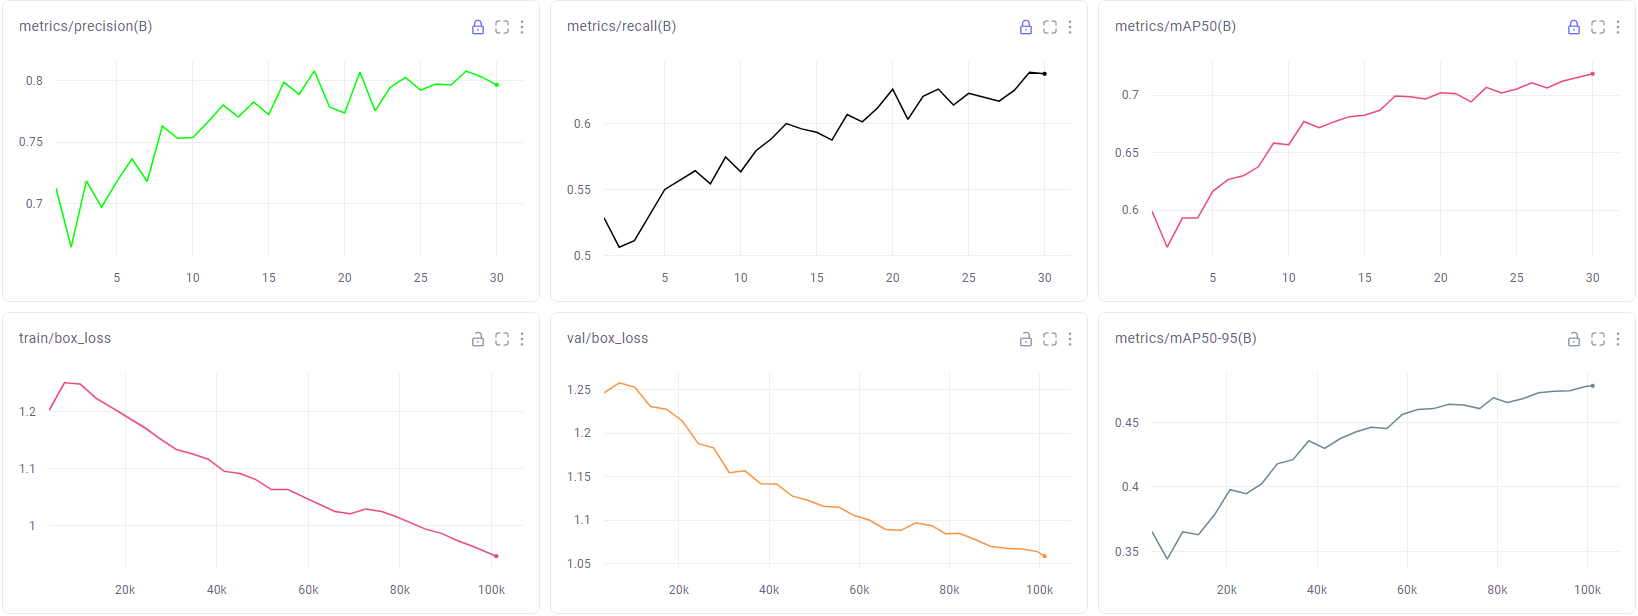
\includegraphics[width=1.0\textwidth]{figures/model}
\caption{Comet.ml dashboard made from the training of our model.}
\label{fig:comet}
\end{figure}

Figure~\ref{fig:comet} depicts the Comet.ml dashboard, which offers a comprehensive representation of the training process,
encompassing loss and accuracy metrics, the learning rate, and the model's performance on the validation set.
This information is vital for evaluating the model's performance and for identifying potential issues that may arise during training.
Furthermore, the Comet.ml platform enables the comparison of different experiments,
which can be beneficial for fine-tuning the model's hyperparameters and for improving its performance.
Which I did try out, for comparing the performances of the same model on the same dataset,
but with different epochs and batch sizes to see and find a good balance between training time and performance.

\subsubsection{Model evaluation}\label{subsubsec:model-evaluation}
The evaluation of the Yolov8 model is performed using a set of metrics that measure its performance on the Cityscapes dataset.
These metrics include precision, recall, mAP, and IoU, which are commonly used in object detection tasks.
I used the mAP metric to evaluate the model's performance on the test set, which provides a comprehensive measure of its accuracy.
The mAP is calculated by averaging the precision-recall curves for each class in the dataset, which gives an overall measure of the model's performance.

\begin{equation}
\text{mAP} = \frac{1}{N} \sum_{i=1}^{N} \text{AP}_i
\end{equation}


where \( N \) is the number of classes and \( \text{AP}_i \) is the average precision for class \( i \).

The IoU metric is used to evaluate the model's ability to accurately predict the bounding boxes for objects in the image.
It measures the overlap between the predicted and ground truth bounding boxes, with a higher IoU indicating a more accurate prediction.

\begin{equation}
\text{IoU} = \frac{\text{Area of Overlap}}{\text{Area of Union}}
\end{equation}


In order to ensure the reliability of the subsequent analysis, only those detections with an IoU value of at least 0.80 were considered,
and only those predictions with a relatively high degree of accuracy were utilised.

The performance of the final and best performing model is evaluated on the test set's all classes averaged:


\begin{table}[h!]
\centering
\begin{tabular}{|c|c|c|c|c|c|c|}
\hline
\textbf{Class} & \textbf{Images} & \textbf{Instances} & \textbf{Box(P} & \textbf{R} & \textbf{mAP@0.5} & \textbf{mAP@0.5:0.95)} \\
\hline
all            & 500             & 10654             & 0.797           & 0.638      & 0.719            & 0.478                 \\
small\_vehicle & 479             & 4832              & 0.889           & 0.751      & 0.834            & 0.604                 \\
person         & 441             & 4095              & 0.829           & 0.651      & 0.738            & 0.445                 \\
large\_vehicle & 141             & 191               & 0.729           & 0.597      & 0.666            & 0.511                 \\
two-wheeler    & 361             & 1536              & 0.741           & 0.553      & 0.637            & 0.354                 \\
\hline
\end{tabular}
\caption{Network performance in all classes, where a detection is a detection with at least 70\% IOU.}
\label{table:performance_metrics}
\end{table}



%Szerintem ide kéne tenni aka tanításos elméleti részról a bekezdés utánna meg a MLOps os részt

